
\documentclass[12pt,a4paper]{article}

% ==================================================
% PACKAGES
% ==================================================

\usepackage[utf8]{inputenc}
\usepackage[T1]{fontenc}
\usepackage[french]{babel}
\usepackage{lmodern}
\usepackage{graphicx}
\usepackage{geometry}
\usepackage{xcolor}
\usepackage{float}
\usepackage{hyperref}
\usepackage{booktabs}
\usepackage{longtable}
\usepackage{setspace}
\usepackage{pdflscape}
\usepackage{rotating}

\geometry{
    top=2.5cm,
    bottom=2.5cm,
    left=2.5cm,
    right=2.5cm
}

\definecolor{ensaiBlue}{RGB}{47,91,140}

\hypersetup{
    colorlinks=true,
    linkcolor=ensaiBlue,
    urlcolor=ensaiBlue
}

\graphicspath{ {./} }

\setlength{\parskip}{0.4em}

\begin{document}

% ==================================================
% PAGE DE GARDE
% ==================================================

\begin{titlepage}
\begin{center}

\IfFileExists{logo_ensai2.jpg}{
    
\includegraphics[width=0.32\textwidth]{logo_ensai2.jpg}
}{
    {\Large \textbf{ENSAI}}
}

\vspace{1.2cm}

{\large
Deuxième année -- Projet informatique
}

\vfill

{\color{ensaiBlue}
\rule{\textwidth}{1.2pt}
}

\vspace{0.7cm}

{\Huge \bfseries ANONYMIA}

\vspace{0.3cm}

{\Large \textbf{Groupe 21}}

\vspace{0.4cm}

{\Large
Application d'anonymisation\\
de documents administratifs
}

\vspace{0.8cm}

{\color{ensaiBlue}
\rule{\textwidth}{1.2pt}
}

\vspace{1.4cm}

{\LARGE \bfseries Rapport final}

\vspace{0.4cm}

{\large
Conception, développement et bilan du projet
}

\vfill

\begin{minipage}{0.75\textwidth}
\centering

{\large \textbf{Équipe projet}}

\vspace{0.5cm}

\begin{tabular}{c}
ALVES Ryan \\[0.2cm]
HAUET Noah \\[0.2cm]
KUATE Cabrel \\[0.2cm]
LE BESNERAIS Tom \\[0.2cm]
LE DOARÉ Tanguy
\end{tabular}

\vspace{1cm}

{\large
\textbf{Tuteur :} LAGALLE Maxence
}

\end{minipage}

\vfill

{\large Année universitaire 2026--2027}

\end{center}
\end{titlepage}

% ==================================================
% TABLE DES MATIÈRES
% ==================================================

\tableofcontents
\newpage

% ==================================================
% 1. CONTEXTE DE L'APPLICATION
% ==================================================

\section{Contexte de l'application}

\subsection{Expression du besoin}

\textit{Section à compléter par le groupe.}

\subsection{Utilisateurs et rôles}

\textit{Section à compléter par le groupe.}

\subsection{Nature et format des données}

\textit{Section à compléter par le groupe.}


% ==================================================
% 2. ARCHITECTURE GÉNÉRALE
% ==================================================

\newpage
\section{Architecture générale}

Anonymia est une application web développée en Python, reposant sur une architecture client-serveur. Elle se compose de deux parties distinctes: une interface utilisateur (\textit{frontend}) et un serveur applicatif (\textit{backend}). Ces deux composants communiquent au moyen de requêtes HTTP. Le backend prend en charge les traitements métier, tandis que le frontend permet à l'utilisateur d'accéder aux fonctionnalités de l'application.

Afin de faciliter la maintenance, les tests et le développement collaboratif, nous avons adopté une architecture en couches fondée sur le principe de séparation des responsabilités (\textit{Separation of Concerns}). Chaque composant possède ainsi un rôle défini et communique avec les autres au travers d'interfaces identifiables.


% --------------------------------------------------
% 2.1 ORGANISATION CLIENT-SERVEUR
% --------------------------------------------------

\subsection{Organisation client-serveur}

Le frontend est développé avec \textbf{Streamlit}, un framework Python permettant de construire une interface web interactive. Il propose notamment la connexion des utilisateurs, le dépôt de documents au format texte, la configuration des paramètres de caviardage et la consultation des résultats.

L'interface ne réalise pas directement les opérations de détection ou de modification des données personnelles. Elle transmet les demandes au backend à l'aide de la bibliothèque \textbf{Requests}. Ces échanges s'effectuent par requêtes HTTP, avec des réponses principalement structurées au format JSON. Lors de l'envoi d'un document, le texte et les paramètres du traitement sont transmis au serveur sous la forme d'une requête multipart.

Le backend est développé avec \textbf{FastAPI} et exécuté par le serveur ASGI \textbf{Uvicorn}. Il expose une API HTTP organisée autour de plusieurs ensembles de routes : l'authentification, la gestion des utilisateurs et le traitement des documents. Il centralise les règles métier, les contrôles d'accès, les opérations de caviardage et les interactions avec les services externes et la base de données.

Cette séparation permet de faire évoluer l'interface sans modifier directement la logique métier. Elle rend également possible l'utilisation de l'API indépendamment du frontend, notamment pour les tests et les opérations de diagnostic.


% --------------------------------------------------
% 2.2 ARCHITECTURE EN COUCHES
% --------------------------------------------------

\subsection{Architecture en couches du backend}

Le backend constitue le cœur de l'application. Son organisation reprend la structure envisagée lors de la phase de conception, en distinguant plusieurs composants complémentaires.

\medskip

\noindent
\textbf{La couche de contrôle} correspond au package \texttt{controller}. Elle constitue le point d'entrée des requêtes HTTP et assure leur transmission vers les services appropriés. Les contrôleurs sont associés à des routes FastAPI, tandis que les modèles du package \texttt{schema}, construits avec Pydantic, définissent et valident la structure des données échangées avec les clients. Cette couche prend également en charge les réponses HTTP et la conversion de certaines erreurs métier en codes de réponse adaptés.

\medskip

\noindent
\textbf{La couche de service}, contenue dans le package \texttt{service}, coordonne les opérations nécessaires à la réalisation des fonctionnalités. Deux classes principales ont été implémentées : \texttt{PersonService}, responsable notamment de l'authentification et des autorisations, et \texttt{DocService}, qui organise le traitement des documents. Cette dernière coordonne les différentes étapes du caviardage, depuis l'analyse du texte jusqu'à l'enregistrement des données associées au traitement.

\medskip

\noindent
\textbf{Les objets métier}, regroupés dans le package \texttt{business\_object}, représentent les entités et les mécanismes propres à l'application. Ils comprennent notamment les objets \texttt{Person} et \texttt{RedactedDoc}, ainsi que les composants chargés de la détection et du caviardage. Ce package contient également les différentes stratégies de traitement du texte. L'utilisation d'objets dédiés permet de séparer les algorithmes des mécanismes de communication HTTP et de persistance.

\medskip

\noindent
\textbf{La couche d'accès aux données}, identifiée par le package \texttt{dao} (\textit{Data Access Object}), assure les échanges avec la base PostgreSQL. Les classes DAO regroupent les requêtes nécessaires à la création, à la consultation et à la modification des informations persistantes. Les connexions sont gérées au moyen de la bibliothèque \texttt{psycopg2}. Cette organisation évite de disperser les requêtes SQL dans les services métier.

\medskip

Enfin, le package \texttt{utils} rassemble plusieurs fonctions transversales, notamment la configuration de l'environnement, la journalisation, la gestion des exceptions et certaines opérations de sécurité. 

Cette décomposition favorise la réutilisation des composants et permet de tester les règles métier indépendamment des contrôleurs HTTP, notamment en simulant les interactions avec la couche DAO.


% --------------------------------------------------
% 2.2.1 DIAGRAMME DE SÉQUENCE
% --------------------------------------------------

\subsubsection{Illustration par un diagramme de séquence}

Afin d'illustrer les interactions entre les différents composants du backend, nous avons réalisé un diagramme de séquence représentant le déroulement de la détection des données personnelles au sein d'un document. Ce diagramme, élaboré lors de la phase de conception, met en évidence le rôle de l'API, du service chargé de coordonner l'analyse et des deux mécanismes complémentaires de détection. Le traitement repose sur l'exécution concurrente du détecteur par expressions régulières et du détecteur utilisant un modèle de langage. Ce dernier fait intervenir des mécanismes de filtrage des entrées et de vérification des réponses produites. Les résultats des deux détecteurs sont ensuite regroupés afin d'obtenir une liste de données personnelles identifiées dans le document.

\begin{figure}[htbp]
    \centering

    \IfFileExists{diagramme_sequence.png}{
        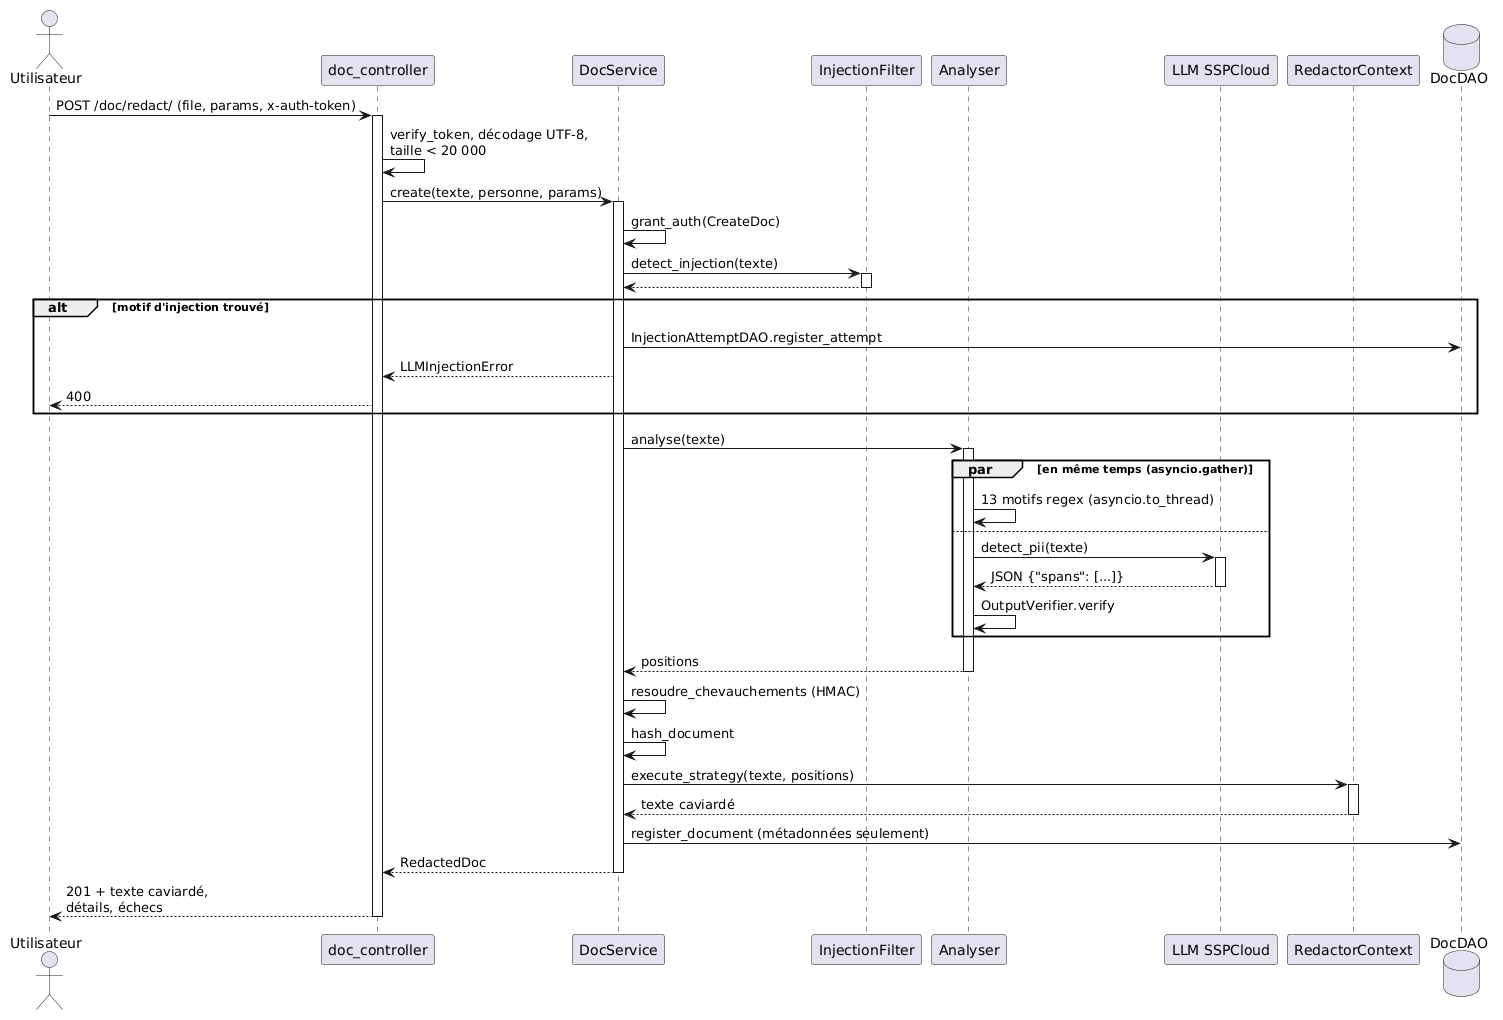
\includegraphics[
            width=\textwidth
        ]{diagramme_sequence.png}
    }{
        \fbox{
            \parbox{0.85\textwidth}{
                \centering
                Diagramme de séquence à insérer.
            }
        }
    }

    \caption{
        Diagramme de séquence du flux nominal
        de détection, issu de la conception initiale
    }
    \label{fig:sequence_detection}
\end{figure}

La figure~\ref{fig:sequence_detection} illustre ainsi le principe de séparation des responsabilités adopté dans notre architecture. Elle se concentre sur la phase de détection, sans représenter l'ensemble des étapes ultérieures de caviardage et de persistance des données. Certains éléments ont évolué depuis cette conception initiale. Dans l'implémentation finale, la coordination du traitement est notamment assurée par \texttt{DocService} et \texttt{AnalyserFactory}, et les détecteurs sont intégrés au moyen des classes \texttt{RegexDecorator} et \texttt{LLMDecorator}. La route de traitement des documents est également devenue \texttt{POST /doc/redact/}.


% --------------------------------------------------
% 2.3 TECHNOLOGIES
% --------------------------------------------------

\subsection{Technologies et composants externes}

Le fonctionnement d'Anonymia repose principalement sur un ensemble de bibliothèques Python spécialisées.

\textbf{FastAPI} assure l'exposition des fonctionnalités du backend sous forme d'API HTTP. \textbf{Pydantic} permet de valider les données échangées, tandis que \textbf{Streamlit} et \textbf{Requests} sont utilisés respectivement pour l'interface web et sa communication avec le serveur.

La persistance est assurée par \textbf{PostgreSQL}. La base conserve notamment les comptes utilisateurs, les informations nécessaires à la gestion des sessions et les métadonnées des traitements. Les documents originaux ne sont pas enregistrés dans les tables de suivi des documents : celles-ci conservent notamment une empreinte du document, la date du traitement et les informations relatives aux données personnelles détectées.

La détection des données personnelles repose sur deux approches complémentaires. Les expressions régulières permettent d'identifier des informations présentant une structure reconnaissable, tandis qu'un grand modèle de langage (\textit{Large Language Model}, LLM) est mobilisé pour analyser les éléments nécessitant une interprétation contextuelle.

L'accès au LLM s'effectue via l'API proposée par \textbf{SSP Cloud}, à l'aide de la bibliothèque Python \texttt{openai} et de son client asynchrone. Cette intégration est indépendante de l'interface utilisateur : les appels au modèle sont déclenchés depuis les composants de détection du backend. Le recours aux fonctionnalités asynchrones de Python permet également d'exécuter les deux mécanismes de détection de manière concurrente.

Enfin, l'environnement d'exécution est géré au moyen de \textbf{uv}, qui facilite l'installation et la synchronisation des dépendances du projet. Les paramètres de connexion et les clés nécessaires aux services externes sont fournis au moyen de variables d'environnement, chargées notamment avec \texttt{python-dotenv}.


% ==================================================
% 3. RÉPONSE AU BESOIN
% ==================================================

\newpage
\section{Réponse au besoin}

\subsection{Introduction}

La réponse précise aux besoins s’est largement axée sur la liste des fonctionnalités obligatoires F1, …, F5 spécifiées dans le sujet. Cependant, nous avons pu commencer à implémenter la fonctionnalité optionnelle FO4. Nous nous attarderons dans cette partie sur le processus central de l’application, c’est-à-dire la détection des données personnelles suivie de l’anonymisation. Bien que les fonctionnalités soient interdépendantes, nous décrirons donc principalement l’implémentation des fonctionnalités obligatoires 2 et 3: détection des données personnelles et anonymisation.


\subsection{Description des fonctionnalités principales}

\subsubsection{Fonctionnalité 2: Détection des données personnelles}

La détection de données personnelles fait en réalité appel à deux processus différents: le premier est la détection de données personnelles par expression régulière. En effet, certaines PII (Personally Identifiable Information) telles que le NIR ou l’IBAN  possèdent des formats connus et encodés de manière prévisible,  ce qui permet  de les détecter à l'aide d'expression régulière. La liste des  PII  est donnée en  annexe. Cependant certaines informations sensibles telles que les prénoms ou les informations médicales ne respectent pas des formats précis. Ainsi, nous pouvons faire appel à des outils plus développés et  pouvant prendre  en compte le contexte  textuel : ce sont les LLM (Large Language Model). Si le LLM rencontre un dysfonctionnement, alors seul la détection par expression régulière est appelée et l’utilisateur en est averti.

Les fonctions de recherche par expression régulière sont disponibles dans la librairie standard de Python. Ainsi, c'est celle-là que nous utiliserons dans notre projet. Cependant, pour accomplir une tâche aussi complexe que la détection de prénom, nous devons utiliser des modèles de langage avancés, qui ne peuvent généralement pas fonctionner sur un ordinateur personnel. Nous faisons alors appel aux modèles de LLM proposés par Onyxia. En particulier, notre application s’est concentrée sur l'intégration du modèle open-source Qwen, et l’API utilisée pour communiquer au LLM utilise le modèle OpenAI, qui est un standard de l’industrie.


\subsubsection{Fonctionnalité 3: Anonymisation}

Nous devons tout d'abord rappeler que l'anonymisation à laquelle nous faisons référence ici n'a aucune valeur juridique. En effet, l'utilisateur reste dans tous les cas responsable du traitement des informations sensibles et l'application ne garantit pas que toutes ces informations seront détectées et caviardées. 
L'anonymisation peut être approchée par deux stratégies: la première est le masquage, et la seconde est l'anonymisation. Le masquage remplace l'information sensible par une référence: par exemple “Jean Martin” est remplacé par "[NOM\_1]". 

La seconde est la pseudonymisation, qui remplace l'information sensible par une information possédant la même forme: par exemple, “Jean Martin” est remplacé par “Paul Durand”. La pseudonymisation que nous pratiquons n'est pas celle au sens du droit RGPD: en effet selon la RGPD, la pseudonymisation implique qu'il est possible de retrouver les informations originales non caviardées; notre application n'enregistre cependant aucune table de correspondance et donc ne permet pas de retrouver les informations sensibles à partir d’un contenu anonymisé.


\subsection{Caviardage d’un document: partie contrôleur}
La première étape de cette fonctionnalité est la soumission d’un document texte. Ceci correspond à la requête \textsc{HTTP post /redact/}. Cette requête contient les paramètres suivants:
\begin{itemize}
\item \textsc{file}: Le fichier à téléverser dans l’objectif d’être caviardé. Plusieurs contraintes s’imposent sur ce fichier: tout d’abord, celui-ci doit être dans un format décodable utf-8 valide. Si cela est le cas, alors il ne doit pas dépasser une certaine longueur pour éviter de surcharger l’application, en particulier de limiter la taille de l’entrée du LLM. Enfin, l’application a été pensée pour des formats en texte brut ou bien proche du texte brut, tel que les formats texte .txt, ou bien le format markdown .md.
\item \textsc{params}: C’est un format JSON, qui a pour attributs les paramètres “llm” et “mask”, tous deux des booléens. “llm” indique si le LLM doit être activé pour cette requête, et le masquage est appliqué dans le cas où “mask” est activé, sinon c’est la pseudonymisation qui est activée. Dans le futur, plusieurs paramètres additionnels pourront être implémentés. 
\item Enfin, bien que cela ne fasse pas partie de la requête elle-même, l'utilisateur doit pouvoir fournir un token valide lui permettant de s'identifier, afin de confirmer que son rôle lui permet de téléverser les documents.
\end{itemize}
\subsection{Caviardage d’un document: partie service}
\begin{landscape}
\begin{figure}[p]
  \thispagestyle{empty}
    \centering
    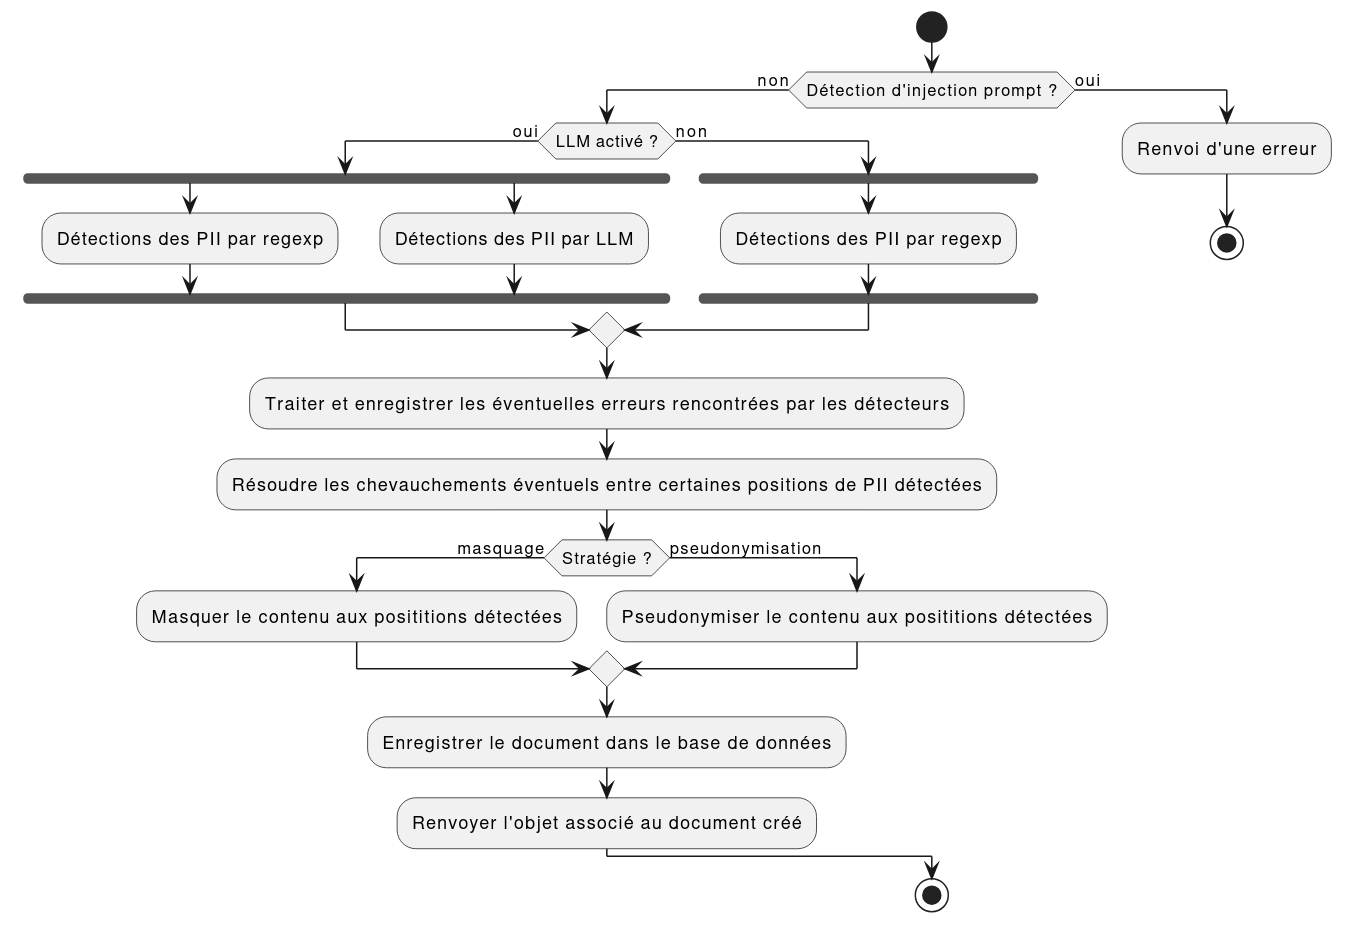
\includegraphics[width=\linewidth,height=0.85\textheight,keepaspectratio]{service}
    \caption{Diagramme d'activité de \textsc{DocService}}
\end{figure}
\end{landscape}
Le service des documents constitue le cœur du processus de caviardage de l’application. Voici le déroulement du processus de création de document:
\begin{itemize}
\item Tout d’abord le service s’assure que l’utilisateur possède la permission de téléverser des documents.
\item Un filtre d’injection est instancié afin de vérifier qu'il n'y a pas de tentative d'injection de prompt dans la requête. Si une tentative d’injection est détectée, alors elle sera enregistrée et rapportée.
\item Suite à cela, le service instancie un “analyseur” (que nous décrirons plus en détail par la suite) qui a pour objectif de  trouver les positions des PII à caviarder à partir d'un texte. Il y a deux processus qui permettent de réaliser cette tâche: d'abord le détecteur par expressions régulières, suivi du détecteur faisant appel au LLM, si celui-ci est activé dans les paramètres spécifiés. Ces deux processus sont exécutés en parallèle afin d'optimiser le temps de réponse de l'application et de se conformer au cahier des charges.
\item Le service fait appel à un “caviardeur” qui s'occupe de remplacer les instances de PII détectées par un contenu masqué ou pseudonymisé en fonction des paramètres spécifiés par l’utilisateur.
\item Le service enregistre le document dans la base de données. On s'assure que le contenu original non caviardé du document n'est pas enregistré
\item Le service renvoie enfin la réponse au contrôleur.
\end{itemize}
\subsection{Détail de l’architecture de l’«Analyseur»}

\begin{figure}[p]
    \centering
    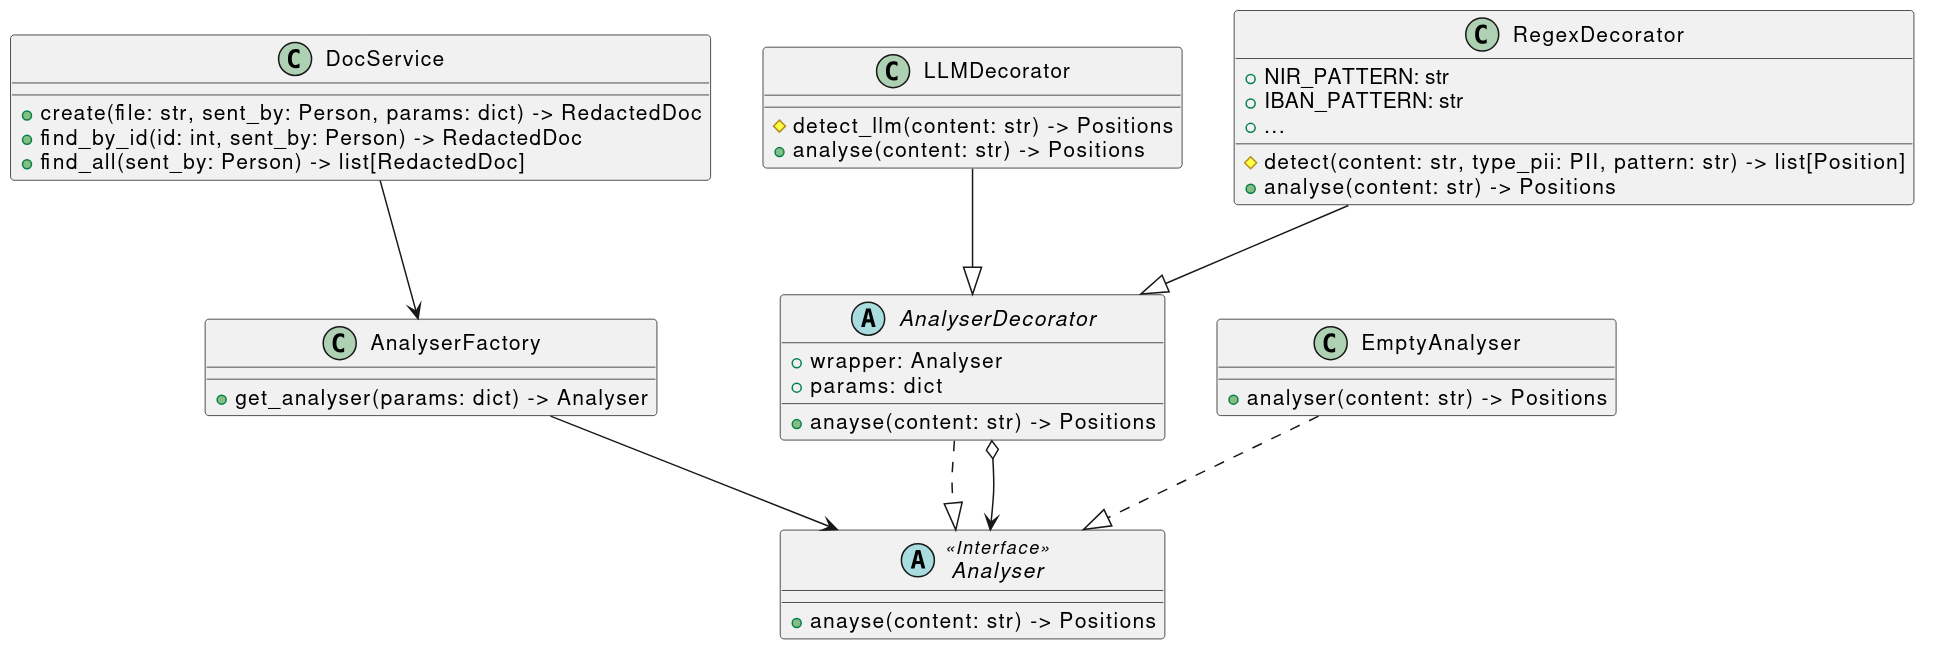
\includegraphics[width=\linewidth]{uml}
    \caption{Diagramme des classes de l'analyseur}
\end{figure}
Le rôle de l'analyseur est central dans le processus de traitement de document. En effet, c'est l'analyseur qui est chargé de prendre en entrée le contenu du fichier téléversé par l'utilisateur et d'en ressortir les positions des PII détectées dans ce document. Cependant, contrairement à \textsc{OutputVerifier} et \textsc{InjectionFilter} ( ayant respectivement pour fonction de s'assurer que la sortie du LLM est valide et que le document téléversé ne contient pas d'injection de prompt), il est implémenté suivant un design pattern plus complexe: c'est le patron du décorateur. Son implémentation est fortement inspirée de l'implémentation proposée par Refactoring Guru. 

\begin{enumerate}
  \item \textsc{Analyseur} est l'interface de base, qui ne possède qu'une fonction virtuelle se chargeant de convertir un contenu textuel en un ensemble de positions de PII.
  \item \textsc{AnalyserFactory} est instanciée par \textsc{DocService}. Elle lit \textsc{params} et assemble la chaîne adéquate.
  \item \textsc{EmptyAnalyser} est l'implémentation de base qui ne renvoie aucune position. Il correspond au composant concret au cœur de la chaîne.
  \item \textsc{AnalyserDecorator} est une classe abstraite qui implémente \textsc{Analyser} et est capable d'envelopper n'importe quel autre analyseur afin de l'appeler dans la chaîne.
  \item Enfin \textsc{RegexDecorator} et \textsc{LLMDecorator} sont les décorateurs concrets. Chacun détecte les PII suivant leurs algorithmes propres et ajoute leur position aux positions déjà produites par le wrapper (le décorateur qu’ils «emballent»).
\end{enumerate}

Le choix du décorateur est motivé par les raisons suivantes:
\begin{enumerate}
  \item Tout d'abord, activer ou non le LLM dépend de params et est donc une donnée runtime; ainsi, le patron permet d’assembler la chaîne à l'exécution.
  \item Les détecteurs sont isolés les uns des autres.
  \item Cela permet une plus grande flexibilité. En effet, en utilisant de l'héritage pur, il y aurait un grand nombre de classes se ressemblant fortement mais possédant une architecture différente à implémenter; cela serait redondant.
  \item Ajouter un maillon dans la chaîne comme par exemple un NLP (Natural Language Processing) ou bien un \textit{LLM as a judge} revient à créer un nouveau décorateur et à ne pas modifier les décorateurs déjà implémentés. Cela permet donc de mieux respecter le principe ouvert/fermé.
  \item Enfin un simple design pattern de stratégie n'aurait pas permis d'implémenter le fait que les détecteurs LLM et Regex sont cumulables.
\end{enumerate}

Enfin, il faut noter que ce principe est tout à fait compatible avec l'exécution asynchrone. Il faut faire attention cependant à lancer les détecteurs Regex par le biais d’un \textit{thread}, car l'implémentation re de la librairie standard python ne fournit pas par défaut de recherche regex en asynchrone. La recherche d’injection de prompt n’a pas été intégrée parmi les décorateurs, car elle s’exécute sur le texte avant le reste de la chaîne. Si la vérification de sortie de LLM (intégrée dans le décorateur LLM) détecte une anomalie, elle renvoie une classe spéciale qui n’est pas un ensemble de positions, mais une classe spéciale (\textsc{AnalysisFail}) qui a pour but de rapporter qu’une erreur s’est produite dans la chaîne, tout en préservant la chaîne.

\subsection{Détail de l’architecture du «Caviardeur»}

\begin{figure}[p]
    \centering
    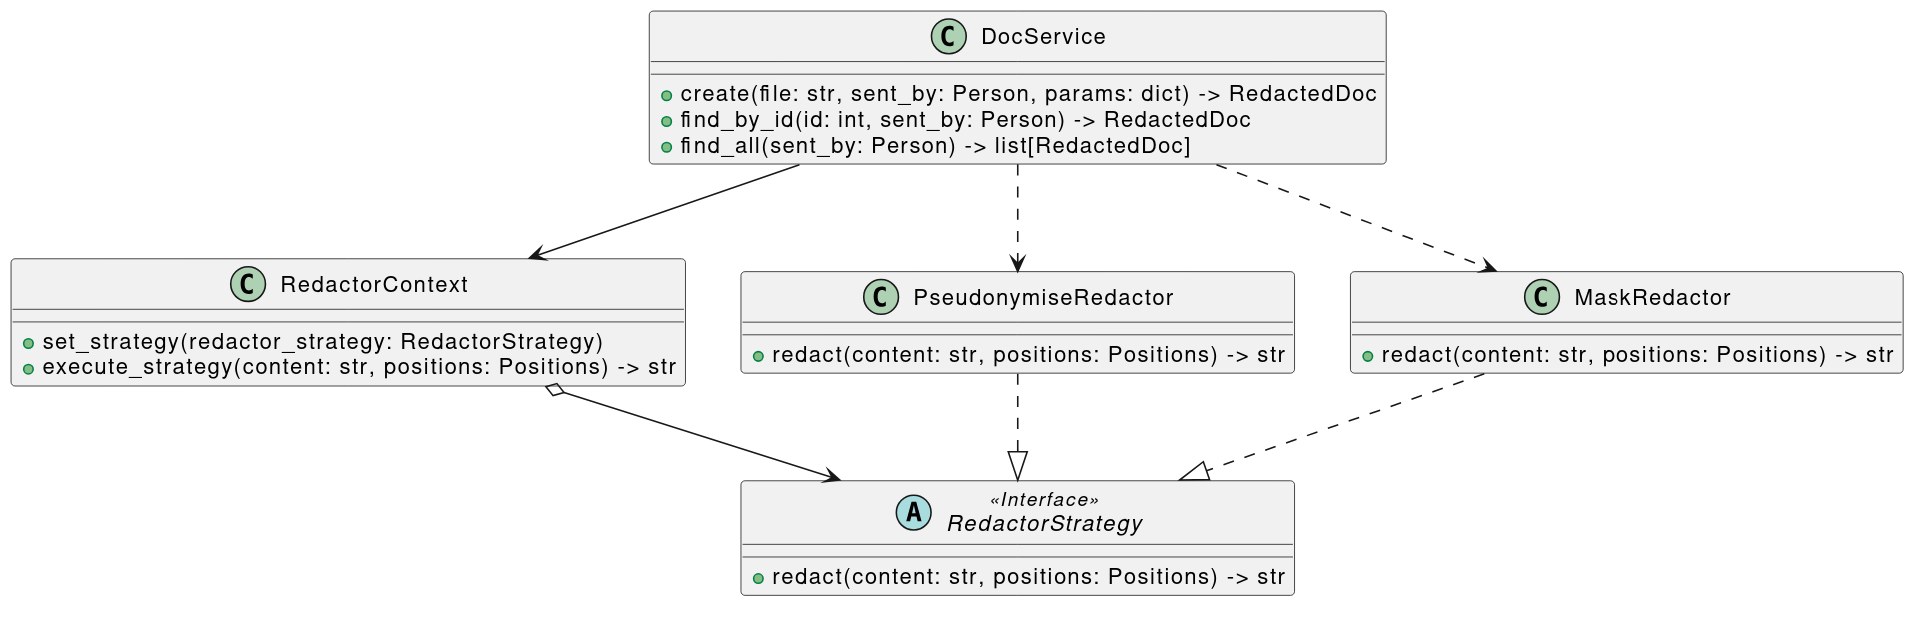
\includegraphics[width=\linewidth]{uml2}
    \caption{Diagramme des classes du caviardeur}
\end{figure}

Une fois la position des PII connues, il existe plusieurs stratégies pour le caviarder: le masquage et la pseudonymisation, que nous avons détaillé précédemment. Cela a été implémenté par le patron de conception de la stratégie, ici aussi fortement inspirée de l’implémentation proposée par Refactoring Guru:

\begin{itemize}
  \item \textsc{RedactorStrategy} (interface) représente le contrat unique, c’est à dire qu’une seule stratégie sera exécutée sur le contenu à caviarder.
  \item \textsc{MaskRedactor} et \textsc{PseudonymiseRedactor} sont les stratégies concrètes, chacune réalisant l'interface.
  \item \textsc{RedactorContext} est le contexte du pattern. Il détient une référence vers la stratégie courante (agrégation, le losange), la change via \textit{set\_strategy}, et la délègue via \textit{execute\_strategy}.
  \item \textsc{DocService} est le client. Il choisit la stratégie (en pointillé vers les deux implémentations, car il les instancie) et la passe au contexte.
\end{itemize}

Le choix du patron est justifié par les raisons suivantes:
\begin{enumerate}
  \item Les algorithmes sont interchangeables. Les deux stratégies ont exactement la même signature d'entrée/sortie. Le client n'a pas besoin de savoir comment le caviardage est fait, seulement lequel demander.
  \item Choix à l'exécution. Le mode de caviardage dépend de params (donc d'une donnée runtime, éventuellement différente à chaque document). Le contexte permet de changer de stratégie sans reconstruire quoi que ce soit.
  \item Principe ouvert/fermé: ajouter un mode (chiffrement réversible, hachage, etc.) revient à créer une nouvelle classe implémentant \textsc{RedactorStrategy}. \textsc{DocService} et \textsc{RedactorContext} ne changent pas.
\end{enumerate}

\subsection{Sécurité}

La sécurité constitue un enjeu central d'Anonymia, puisque l'application est amenée à manipuler des documents contenant potentiellement des données personnelles sensibles. Elle concerne à la fois la protection des compte utilisateurs, la conservation des données traitées et la sécurisation de
l'utilisation du modèle de langage.

Concernant l'authentification, les mots de passe des utilisateurs ne sont jamais stockés en clair dans la base de données. Seule une version hachée et salée est conservée, de sorte qu'une compromission de la base ne permette pas d'accéder directement aux mots de passe. Les droits d'accès sont également limités selon trois rôles : utilisateur, superviseur et administrateur. Cette séparation permet de restreindre l'accès aux fonctionnalités sensibles, notamment la gestion des comptes et la consultation de l'historique des traitements.


Une attention particulière est également portée aux documents soumis à l'application. Le contenu brut d'un document n'a pas vocation à être enregistré de manière permanente. La journalisation conserve uniquement les métadonnées nécessaires au suivi du traitement, telles que l'utilisateur, la date, les détecteurs utilisés ou le nombre de PII détectées. Une empreinte cryptographique du document peut également être calculée afin de pouvoir identifier qu'un document a déjà été traité sans avoir à conserver son contenu. De plus, pour rendre le caviardage cohérent (par exemple “Jean Dupont” toujours caviardé en “[NOM\_1]”, et pas “[NOM\_1]”, puis “[NOM\_2]”), les stratégies de caviardage doivent enregistrer des tables de correspondanc. Pour que le masquage ne puisse pas être inversé, les stratégies de caviardage sont instanciées seulement au runtime, et chaque document a sa propre instance de “caviardeur”, ce qui rend impossible la réversibilité. 

L'utilisation d'un LLM introduit par ailleurs un risque spécifique d'injection de prompt. Un document soumis par l'utilisateur peut contenir des instructions malveillantes afin de pousser le modèle à ne pas détecter certaines PII. Si une telle attaque réussissait, des données personnelles pourraient rester présentes dans le document final. Pour limiter ce risque, Anonymia repose sur une défense en profondeur en trois étapes: 

\begin{enumerate}
\item Tout d'abord, un prompt système strict rappelle au modèle que le document constitue uniquement une donnée à analyser et que les instructions qu'il contient ne doivent pas être exécutées.
\item Ensuite, un \textsc{InjectionFilter} recherche avant l'appel au LLM des motifs susceptibles de correspondre à une tentative d'injection.
\item Enfin, la sortie du modèle est contrôlée par un \textsc{OutputVerifier}, qui vérifie le respect du format attendu, la validité des types de PII retournés ainsi que la présence réelle dans le document des éléments signalés par le modèle.
\end{enumerate}

Aucune de ces protections n'étant suffisante isolément, leur combinaison permet de réduire le risque d'une sortie incorrecte ou manipulée. Le détecteur Regex constitue également un niveau de sécurité supplémentaire, puisqu'il ne dépend pas des instructions présentes dans le document. En cas d'échec ou d'indisponibilité du LLM, l'application peut ainsi continuer à fonctionner en mode dégradé à partir des résultats issus des expressions régulières, et en avertir l’utilisateur.

% ==================================================
% 4. OUTILS MIS EN PLACE
% ==================================================

\newpage
\section{Outils mis en place}

\subsection{Organisation et collaboration}

\textit{Présenter Git, GitHub, VS Code,
Onyxia, Overleaf et les outils de communication.}

\subsection{Environnement technique}

\textit{Présenter PostgreSQL, uv,
les variables d'environnement et la journalisation.}

\subsection{Tests et validation}

\subsubsection{Tests DAO}

\textit{Section à compléter.}

\subsubsection{Tests des services}

\textit{Section à compléter.}

\subsubsection{Audit et tests complémentaires}

\textit{Présenter les résultats des tests
et les corrections apportées.}


% ==================================================
% 5. CHOIX DE CONCEPTION
% ==================================================

\newpage
\section{Choix de conception}

\subsection{Gestion des utilisateurs et des droits}

\textit{Section à compléter.}

\subsection{Protection et conservation des données}

\textit{Section à compléter.}

\subsection{Choix des patrons de conception}

\textit{Présenter notamment Decorator et Strategy.}

\subsection{Gestion des erreurs et mode dégradé}

\textit{Section à compléter.}


% ==================================================
% 6. CONCLUSION
% ==================================================

\newpage
\section{Conclusion et perspectives}

\textit{Présenter le bilan du projet,
les limites rencontrées et les améliorations possibles.}


% ==================================================
% 7. NOTES INDIVIDUELLES
% ==================================================

\newpage
\section{Notes individuelles}

\subsection{Ryan Alves}

\textit{Note individuelle -- une page maximum.}

\subsection{Noah Hauet}

\textit{Note individuelle -- une page maximum.}

\subsection{Cabrel Kuate}

\textit{Note individuelle -- une page maximum.}

\subsection{Tom Le Besnerais}

\textit{Note individuelle -- une page maximum.}

\subsection{Tanguy Le Doaré}

\textit{Note individuelle -- une page maximum.}

\end{document}

